
\documentclass[journal]{IEEEtran}
\usepackage{lipsum}
\usepackage{tikz}
\usetikzlibrary{decorations.pathreplacing,angles,quotes}

% correct bad hyphenation here
\hyphenation{op-tical net-works semi-conduc-tor}

\begin{document}
%
% paper title
\title{Paper Discussion Report}

% puts info about authors at bottom of first page
\author{Lawrence~Owusu,~Jordan~Sturtz,~and~Swetha~Chittam~% <-this % stops a space
  \thanks{The authors are graduate students at NCA\&T}% <-this % stops a space
}

% note the % following the last \IEEEmembership and also \thanks -
% these prevent an unwanted space from occurring between the last author name
% and the end of the author line. i.e., if you had this:
%
% \author{....lastname \thanks{...} \thanks{...} }
%                     ^------------^------------^----Do not want these spaces!

% The paper headers
% The only time the second header will appear is for the odd numbered pages
% after the title page when using the twoside option.
\markboth{CS851 - Deep Learning: Paper Discussion Report}%
{Shell \MakeLowercase{\textit{et al.}}: CS851 - Deep Learning: Method Discussion Report}

% make the title area
\maketitle

% As a general rule, do not put math, special symbols or citations
% in the abstract or keywords.
% \begin{abstract}
% The abstract goes here.
% \end{abstract}

% Note that keywords are not normally used for peerreview papers.
% \begin{IEEEkeywords}
% IEEE, IEEEtran, journal, \LaTeX, paper, template.
% \end{IEEEkeywords}

% For peer review papers, you can put extra information on the cover
% page as needed:
% \ifCLASSOPTIONpeerreview
% \begin{center} \bfseries EDICS Category: 3-BBND \end{center}
% \fi

%
% For peerreview papers, this IEEEtran command inserts a page break and
% creates the second title. It will be ignored for other modes.
\IEEEpeerreviewmaketitle

\section{Summary}

%
% Here we have the typical use of a "T" for an initial drop letter
% and "HIS" in caps to complete the first word.
\IEEEPARstart{A}{} paper authored by Gunasekaran, et al. (2021) uses deep learning methods 
to perform classification of viruses from their DNA sequences. Since DNA is composed of strings
of nucleotides, the problem amounts to classifying viruses according to samples of nucleotide
strings. The authors collect data from the public nucleotide sequence database,
The National Centre for Biotechnology Information (NCBI) https://www.ncbi.nlm.nih.gov.
They then encode this data using label encoding and kmer encoding. For each encoding type,
they run three different deep learning models: CNN, CNN-LSTM, and CNN-Bidirectional-LSTM.
The architectures of all three models start with embedding layers, then convolutional layers,
then max pooling layers, and then from there diverge to either add LSTM layers or 
bidrectional LSTM layers before finishing with dense layers and a final output layer.
The authors compare all six combinations of the two encoding methods with the three model types
using several performance metrics.

\section{Problem Statement}
All DNA and RNA is composed of a string of nucleotides. A nucleotide refers to one of
four compounds for DNA (adenine, cytocine, guanine, thymine) or four compounds for RNA
(adenine, cytocine, guanine, uracil). For double-helix DNA or RNA, each nucleotide
bonds with one and only one other nucleotide, forming what is called a base pair (fig 1). Since
these base pairs are fixed, then, a DNA or RNA sequence can be identified solely by one
side of the double helix. Thus, every DNA virus can be identified by a single string of
characters drawn from the set $\{A, C, G, T\}$ and every RNA virus can be identified by a string
of characters drawn from the set $\{A, C, G, U\}$. The task, then, is to build highly accurate
models to classify a virus from its DNA or RNA sample.

\begin{figure}[h]
  \centering
  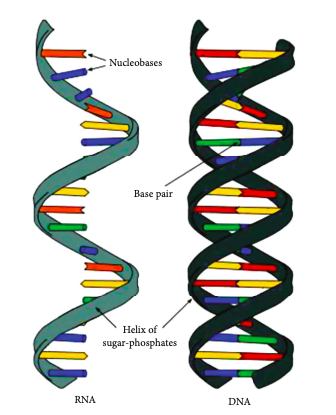
\includegraphics[width=8cm]{figures/dna.png}
  \caption{Single or double-stranded DNA/RNA}
\end{figure}

\section{Related Work}
\lipsum[1] % Generate latin nonsense

\subsection{Current Results on Proposed Problem}
\lipsum[1] % Generate latin nonsense

\section{Data Collection}
The authors obtain complete genomic sequences from the 
National Centre for Biotechnology Information (NCBI) https://www.ncbi.nlm.nih.gov/.
Sequence length ranges from 8 to 37971 nucleoids. They collected genomic sequences
for six virus classes: COVID, MERS, SARS, Dengue, Hepatitus, and Influenza (Fig 2).
Because the population of these viruses were unbalanced--for instance, there were 37272
samples of COVID and only 1418 samples of MERS--the authors opted to use
Synthetic Minority Oversampling Technique (SMOTE) to get a more even distribution of
all six classes in their dataset.

\begin{figure}[h]
  \centering
  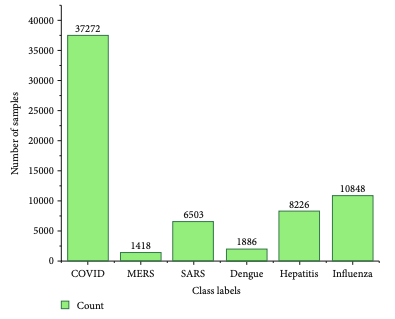
\includegraphics[width=8cm]{figures/data_collection.png}
  \caption{Samples of virus classes retrieved from NCBI}
\end{figure}

\section{Data Preprocessing}
The authors encoded the data in two different formats for comparative analysis.
In the first approach, they use label encoding, which replaces each nucleoid by a unique index value,
preserving positional information (fig 3).
In the second approach, they used kmer encoding, which generates all kmers from a sequence 
and forms an English-like sentence onto which natural language processing techniques
can be applied (fig 4).

\begin{figure}[h]
  \centering
  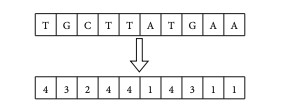
\includegraphics[width=8cm]{figures/label_encoding.png}
  \caption{Label encoding example}
\end{figure}

\begin{figure}[h]
  \centering
  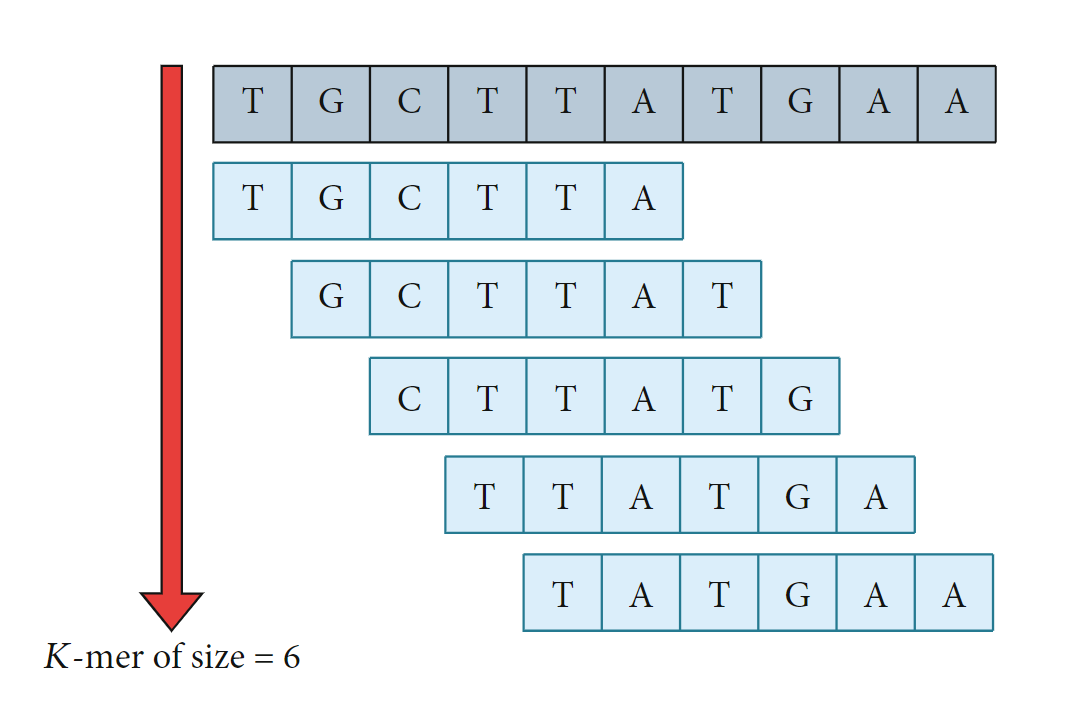
\includegraphics[width=8cm]{figures/kmer_encoding.png}
  \caption{Kmer encoding example, where k=6}
\end{figure}

Once encoded, in both cases the input data is one-hot encoded and then fed into
the first layer of the models, which is an embedding layer.

\section{Proposed Models}
\lipsum[1] % Generate latin nonsense

\subsection{Model Architecture}
\lipsum[1] % Generate latin nonsense

\subsection{Model Parameters}
\lipsum[1] % Generate latin nonsense

\section{Paper Results}
\lipsum[1] % Generate latin nonsense

\subsection{Comparison Results}
\lipsum[1] % Generate latin nonsense

\section{Conclusion}
\lipsum[1] % Generate latin nonsense

\begin{thebibliography}{1}

\bibitem{IEEEhowto:kopka}
H.~Gunasekaran, K.~Ramalakshmi, A.~Rex~Macedo~Arokiaraj, S.~Deepa~Kanmani, C.~Venkatesan, and C.~Suresh~Gnana~Dhas.
  "Analysis of DNA Sequence Classification Using CNN and Hybrid Models." 
  \emph{Computational and mathematical methods in medicine}, 2021.
\end{thebibliography}

\end{document}
